\documentclass[11pt]{article}

\usepackage{amssymb,amsmath,amsfonts,eurosym,geometry,ulem,graphicx,caption,color,setspace,sectsty,comment,footmisc,caption,natbib,pdflscape,subfigure,array,hyperref,epigraph,multirow,tabu}

\usepackage[T1]{fontenc}
\usepackage[utf8]{inputenc}
\usepackage{tgpagella}
\usepackage{todonotes}
\usepackage{textcomp}
\usepackage{eurosym}

\normalem

\onehalfspacing
\setlength{\parskip}{0.3em}

\newtheorem{theorem}{Theorem}
\newtheorem{corollary}[theorem]{Corollary}
\newtheorem{proposition}{Proposition}
\newenvironment{proof}[1][Proof]{\noindent\textbf{#1.} }{\ \rule{0.5em}{0.5em}}

\newtheorem{hyp}{Hypothesis}
\newtheorem{subhyp}{Hypothesis}[hyp]
\renewcommand{\thesubhyp}{\thehyp\alph{subhyp}}

\newcommand{\red}[1]{{\color{red} #1}}
\newcommand{\blue}[1]{{\color{blue} #1}}

\DeclareMathOperator*{\argmax}{arg\,max} 

\newcolumntype{L}[1]{>{\raggedright\let\newline\\arraybackslash\hspace{0pt}}m{#1}}
\newcolumntype{C}[1]{>{\centering\let\newline\\arraybackslash\hspace{0pt}}m{#1}}
\newcolumntype{R}[1]{>{\raggedleft\let\newline\\arraybackslash\hspace{0pt}}m{#1}}

\geometry{left=1.0in,right=1.0in,top=1.0in,bottom=1.0in}

\begin{document}

%+Title
\title{%
\textbf{Mapping Research \& Innovation Missions \\
\large With an application to the UK Government Mission to transform the prevention, diagnosis and treament of chronic diseases using Artificial Intelligence}}
\author{Juan Mateos-Garcia}
%\date{}
\maketitle
%-Title
%+Abstract
\begin{abstract}
Mission-oriented innovation policies to address specific technological, social or economic challenges are being increasingly recognised as a promising strategy to steer innovation in societally desirable directions and encourage the formation of new disciplines and industries. The formulation of this policy agenda has however raced ahead of the evidence base, creating the risk that mission-oriented innovation policies are insufficiently informed in their formulation, targeting, monitoring and evaluation. We argue that developing a suitable evidence base for mission-oriented policies will require the use of new data sources, analytical methods and indicators that reflect their rationale and pathways to impact through network-building and interdisciplinary crossover, and help manage the risks of capture and `picking winners' prematurely. We deploy these methods to develop prototype indicators in the empirical setting of the UK government Grand challenge to \textit{`Use data, Artificial Intelligence and innovation to transform the prevention, early diagnosis and treatment of chronic diseases by 2030`}. Having identified an `active mission field' of projects that combine AI and chronic disease-related keywords, we show that although chronic diseases are underrepresented among AI projects, this situation has started to change in recent years, with fast growth in the active mission field. We also find that projects in the active mission field tend to generate more technological outputs, combine various disciplines, and involve younger specialist organisations. We conclude with an experimental analysis of the `trajectories' of the active mission field using a hierarchical topic modelling approach, and show that topics related to AI tend to be more prevalent that topics related to chronic diseases in the active mission field, suggesting that the exploration of technological opportunities is being driven by computer scientists rather than medical scientists and biotechnologists. Having said this, the diversity of trajectories being explored in the active mission field has not decreased over time, consistent with the idea that it is not settling prematurely into a dominant `solution' for its challenge. We hypothesise that is a consequence of the diversity of funders participating in the area. 
\end{abstract}
%-Abstract

\section{Introduction}
\label{sec:introduction}

Mission-oriented Research \& Innovation policies are systemic public policies that draw on frontier knowledge to attain specific goals or `big science deployed to meet big problems' (Mazzucato, 2018). Missions are at the core of new €100bn EU proposal for Horizon Europe (released June 2018), and of the new industrial strategy developed by UK government, which is organised around the idea of `Grand Challenges’ that generate missions, as well as an `Industrial Strategy Challenge Fund’ that identifies particular challenges to be pursued through concerted policy action (HM Government, 2018). Some mission ideas and policies include \textit{`Reach net zero greenhouse gas emissions balance of 100 European cities
by 2030'} (Mazzucato, 2018), or \textit{`Ensure that people can enjoy at least 5 extra healthy, independent years of life by 2035, while narrowing the gap between the experience of the richest and poorest'} (BEIS, 2018). The figure below illustrates a mission specification from Mazzucato (2018).

\begin{figure}[!ht]
    \centering
    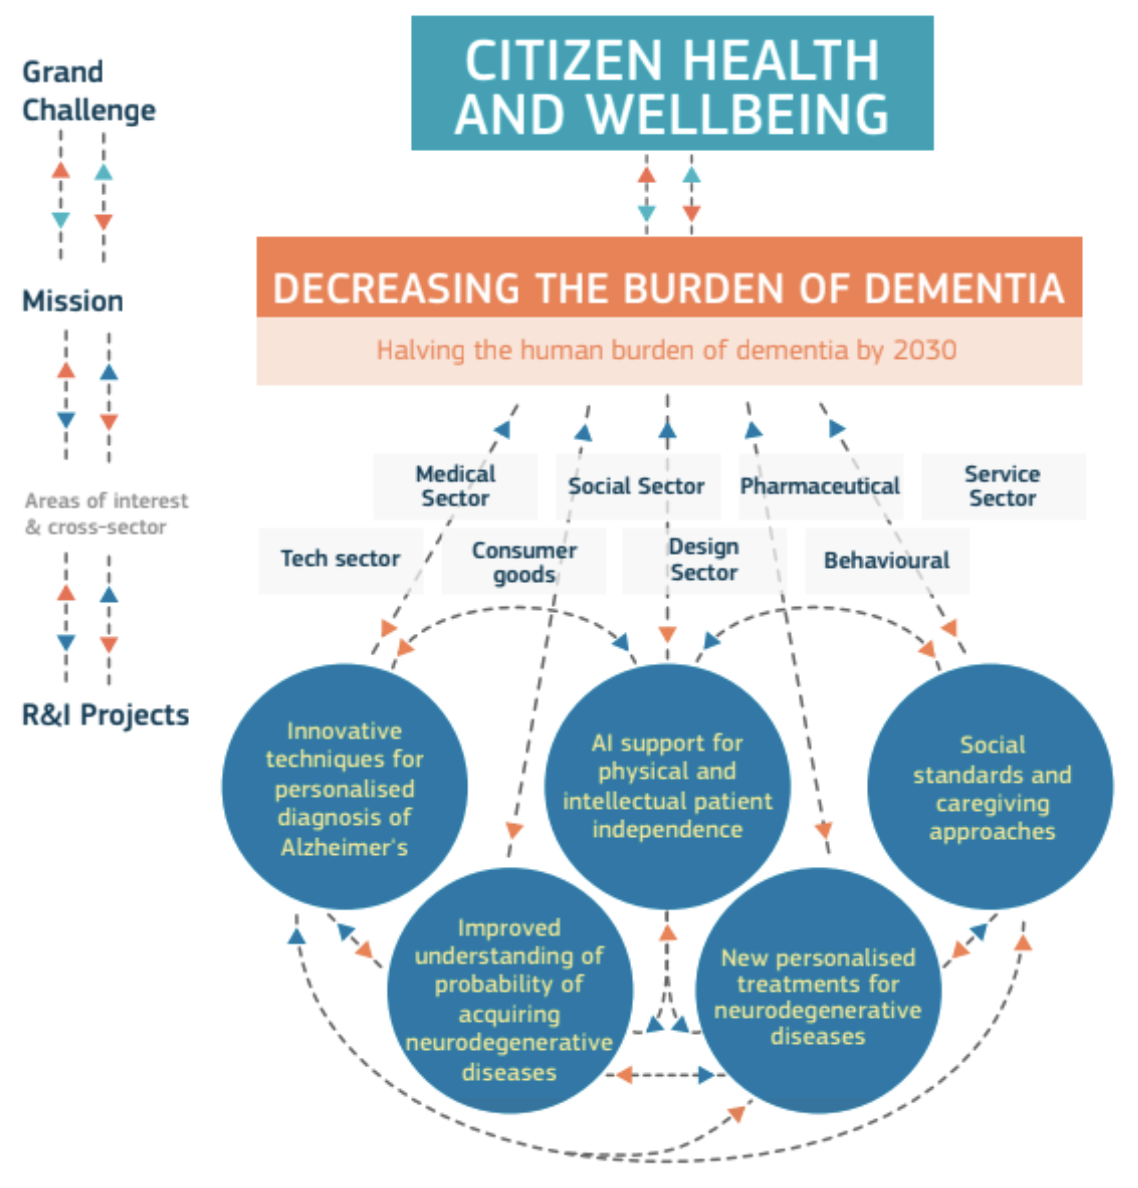
\includegraphics[width=0.8\textwidth]{figures/fig1_example.png}
    \caption{Example mission}
    \label{fig:my_label}
\end{figure}

Missions could help bridge worrying disconnects between technology development, societal well-being and productivity growth by actively encouraging the deployment of new technologies to tackle societal challenges and supporting the exploration of new technological trajectories where `new ideas are less hard to find' (\todo{add ref} Bloom etc). At the same time, missions present important risks: they could fail to target the most significant societal challenges resulting in a loss of legitimacy for their administrators and R\&I policy more widely, they may be unrealistic or unfeasible, or `pick winners' that are commercially unsustainable, rent-seeking or induce premature lock-in to weaker technologies. 

Realising the potential of missions while managing these risks requires a suitable evidence base and indicators for policy prioritisation, targeting, monitoring and evaluation. In this paper, we seek to contribute to this evidence base by developing prototype indicators in the domain of one particular mission \- the mission to transform the prevention, diagnosis and treatment of chronic diseases using `Artificial Intelligence, Data and Innovation' announced by UK Government in 2018. In doing this, we explore the potential of unstructured data and data science methods for generating relevant and inclusive indicators for R\&I policies increasingly concerned with the deployment of emerging technologies in specific directions. 

In the rest of this section, we review the literature about mission-oriented R\&I policies, highlighting their characteristics, rationales, risks and evidence needs, and outline the goals of the paper as well as our research questions. Having done this, in Section \ref{sec:methodology} we describe our methodology, including data collection, processing and enrichment activities, and the approach we have used to operationalise our focus mission in order to generate indicators about it. Section \ref{sec:findings} presents our findings and \ref{sec:conclusion} ends with a discussion of the implications of our analysis, its limitations and issues for further research.

\subsection{A brief history of missions}
\label{subsec: history}

Missions are not new in R\&I policy. Some of humankind`s greatest technical achievements have resulted from missions. Some examples include the Longitude Reward, which encouraged the development of sea watches greatly improving the safety of sea travel in the 18th Century, the Manhattan Project to develop an atomic bomb, or the Apollo program to put a man on the moon (Mowery, Nelson, \& Martin, 2010; Nelson, 1977). Mission-like policies also play an important part in the private sector through crowdsourcing challenges and competitions (a comparative assessment of some of the biggest and most influential frameworks can be accessed \todo{add links} here). 

One thing that sets the `new wave' of missions in R\&I policy apart from previous ones is their shift away from purely technical or economic problem\-solving, and their ambition to deploy science and technology to address big social challenges that people face in their daily lives. One implicit goal of this effort is to build popular support for R\&I policies that can otherwise feel removed from everyday aspirations and concerns about the environment, health, education and inequality (Mazzucato, 2018b). This move away from technical goals to social ones creates new challenges for R\&I policy and its stakeholders, as the goal of
innovation research and policy shift from advancing knowledge and producing technical breakthroughs to achieving social changes which are harder to measure and in some cases even contested, as we see in ongoing debates about how to tackle climate change or increase social mobility (Nelson, 1977, 2011). This broader and arguably more ambitious definition of missions also requires engaging a wider set of disciplines, overcoming barriers to interdisciplinary collaboration.

Another important reason for renewed interest in the mission framework is the notion that traditional R\&I policies based on market failure and system failure rationales ignore the directionality of technical change, have low additionality and tend to be captured by the status quo (Cantner \& Vannuccini, 2018; Frenken, 2017). In other words, they support incremental activities that might not be the most societally desirable, and in some cases would have been carried out anyway, generally by powerful, established incumbents (Frenken, 2017). 

This way of thinking about the goals of R\&I policy draws on evolutionary economics and complexity science ideas suggesting that technological development is directional (it can unfold in multiple possible trajectories) and uncertain in outcomes (the trajectory that is selected ‘from the bottom up’, for example by market forces might not be the most beneficial one because it generates unanticipated externalities and path dependencies that prevent shifts away from it further down the line, as we see in the economy’s lock-in to environmentally unsustainable fossil fuels) (Aghion, David, & Foray, 2009; Arthur, 2009; David, 1985). Further. ‘normal’ R&I takes place through an exploration of the ‘adjacent
possible’ where bodies of knowledge that are technically closer tend to be recombined more often because they exist in the same organisation, or in related organisations (Boschma, 2005; Hidalgo et al., 2018). All this means that R\&I policies that simply seek to increase the amounts invested in R&D (as R\&D tax credits do under a market failure rationale) or the responsiveness of academic researchers to industry needs (as knowledge exchange programs informed by a systems failure rationale do) will fail to generate societally beneficial,
boundary spanning innovations (Gustafsson & Autio, 2011). 

Recent criticisms of mainstream science policy, research funding in the biomedical domain, and the emphasis of AI research on automating labour instead of complementing it, and evidence of a productivity puzzle where increasing investments on R\&D fail to produce corresponding improvements in productivity growth and societal well\-being are consistent with this view (Acemoglu \& Restrepo, 2018; Jones & Wilsdon, 2018; Restrepo & Acemoglu, 2018; Sarewitz, 2016).

A mission-driven R&I framework could help address these challenges: by definition, missions are directional. They identify preferred trajectories of technological development (in the examples we provided at the beginning, use of urban infrastructure and built space innovations to reduce carbon emissions, or of AI to address chronic diseases) and provide resources for pursuing them. They also involve combinations of knowledge residing in faraway parts of the innovation system. This should yield new ideas for which there is not a market yet (otherwise they would already be deployed to address the mission) (Autio, 2011). This could involve new players sitting in the intersection between disciplines, and with a greater tolerance for risk. As before, the ambitions of this new approach come with their own challenges, such as the risk that R\&I policymakers without sufficient information end up trying to `pick winners’ that are not feasible or commercially sustainable, or that they are captured
by new constituencies that coalesce around missions (Aghion et al., 2009). Proponents of the new wave of mission-driven policies set out to address these design and implementation challenges by putting in place new criteria for mission selection of delivery (see table 1) (Mazzucato, 2018b).

\begin{table}[!]
\centering
\begin{tabu} to \textwidth {  X[c]  X[c]  X[c]  }
 \\
 \\
 \textbf{Mission selection criterion} & \textbf{Feature of the evidence base} & \textbf{Indicators}
 \\
 \hline
 \\
 \textbf{1. Social relevance:} Missions should be bold, inspirational and with wide societal relevance & 
 Measure social relevance and engagement with the mission   
 & Alignment of mission objective and expressions of societal need Social media engagement with the mission
 \\
 \\
 \textbf{2. Feasible distinctiveness}: Ambitious but realistic R\&I activities
 & Measure the extent to which the activities being supported draw on but are qualitatively different from previous research.
 & Distinctiveness/relatedness between mission activities and the status quo
 \\
 \\
 \textbf{3. Induces crossover:} Cross-disciplinary, cross-sectoral, and crossactor
 & Measure if the mission is encouraging new combinations of disciplines, technologies and industries
 & Disciplinary diversity in missions compared to status quo and novelty of mission participants compared to the `status quo'.
 \\
 \\
 \textbf{4. Diverse solutions:} Multiple, bottom-up solutions.
 & Measure the diversity of options that are being explored as part of the mission.
 & Diversity of approaches in the mission field
 \\
 \\
 \textbf{5. Measured Clear direction:} measurable, time-bound Measure if the R\&I activities taking place as part of the mission are achieving its goals
 & Design features of the mission (KPIs, duration)
 & Attribution of impacts to mission activities
 \\
 \\
 \hline
\end{tabu}
\caption{Mission goals, measurements and indicators}
\end{table}

\subsection{Developing an evidence base for missions}
\label{subsec:evidence}

These criteria seek to ensure that missions have legitimacy and broad social support, can be achieved, and bring together a broad mix of actors going beyond `the usual suspects'. The demand for bottom-up experimentation acknowledges uncertainty about which of the avenues that are explored through the mission will be successful, and to avoid the risk of picking winners that end in a technological or commercial dead-end. Effective design, delivery, monitoring and evaluation of missions requires a suitable evidence base. We draw on the criteria above to sketch some features of this evidence base, and identify new opportunities to develop new indicators to make it operational (see table 1):

First, an evidence base for missions should capture the extent to which the topic of a mission reflects societal interests and concerns, as well as the levels of social engagement with the mission topic, and with the mission itself. It is possible to generate indicators capturing the social relevance dimension of missions with data from opinion surveys, policy debates, news media and social media. 

Second, the evidence base needs to consider the content of the R\&I activities taking place as part of the mission, and how they balance feasibility (the activities taking place need to be technologically plausible and possible) and ambition (the activities would not have taken place without the mission). This can be measured with indicators reflecting the semantic similarity (or distance) between R&I activities taking place as part of the mission and previous work, as well as the extent to which the projects taking place inside the mission
generate technological outputs (i.e. are technologically feasible).

Third, it is also important to consider the diversity of activities that are being supported through the mission in terms of the disciplines, industries and actors involved: are these novel and unexpected, and do they involve new `entrants’? Here we can develop indicators measuring the disciplinary and industry mix of the activities supported by a mission, and compare the actors participating in it with those involved in areas outside of the mission. Over time, we would expect successful missions to change the structure of R&I networks, bringing key disciplines and the actors involved in them into new fields and communities. We can develop indicators that capture this.

Finally, the evidence base should capture the time\-lines and goals for the mission: what does it seek to achieve, over what period, and with what success. Some of the relevant indicators can be directly extracted from the specification of the mission (eg. reach zero greenhouse emissions by 2030). This is a different question from whether these indicators are being measured in a suitable way, and from the extent to which changes in those indicators (impacts) can be attributed to the mission itself (as compared to broader socio-economic trends and technological breakthroughs supported outside of the mission). This will require experimental designs that will depend on the nature of the mission, its goals and available data.

\subsection{About this paper}
\label{subsec: about}

This paper explores potential indicators to operationalise key dimensions of the evidence base for missions outlined above. We do this in the context of the UK Grand Challenge Mission to \textit{`Use data, Artificial Intelligence and innovation to transform the prevention, early diagnosis and treatment of chronic diseases by 2030'}, and using data about research funding in the UK from the Gateway to Research open dataset. Our goal is to develop a flexible framework that can be used to query funding data and identify a `mission field'. We define a mission field as the set of R&I activities that are directly relevant for a mission. We establish relevance using a semantic approach that extracts keywords from the definition of a mission and then queries the funding corpus with a version of that keyword set expanded via semantic similarity in a word embedding space. We then calculate indicators in the mission field. All these activities are described in further detail in the Methodology and Findings sections below.

We focus on dimensions 2, 3, and 4 in Table 1, considering actors, activities and networks but not impacts and social media activity (see figure below for a summary). The reason for this is that mission-driven innovation policies are a novel policy concept and most missions (including the one we are focusing on in this paper) have only been recently implemented. It would be unrealistic to expect them to have produced visible impacts so early after launch. 

We consider some options for this (challenging) form of mission-driven policy monitoring and evaluation in the conclusions. 

At the onset of the paper we decided to concentrate on the GtR data, which is why we have not used social media data in the analysis.

A next step for us will be to integrate it into our pipeline, possibly through the CrossRef Event API, which allows querying of research paper Document Object Identifiers (DOI) to identify social media activity around them (Ortega, 2018).

The previous point about the nature of the phenomenon we are capturing at this point in time also applies to the actor, activity and outcome indicators that we are focusing on in the paper \- that is to say, the levels of activity we are capturing in our analysis should be seen as a `baseline' for the mission rather than evidence of its impact, given the short time that the mission has had to change the orientation and configuration of R&I activities.

\subsection{Current focus and potential extensions}
\label{subsec: domain}

Our application domain are publicly funded R&I activities in the UK related to the application of Artificial Intelligence (AI) and data to the prevention, diagnosis and treatment of chronic diseases. The idea underlying this mission is that general purpose AI (and machine learning) technologies with high predictive potential could be deployed to transform how we deal with chronic conditions such as cardiovascular diseases, cancer or diabetes (Cockburn, Henderson, \& Stern, 2018; Loder \& Nicholas, 2018).1 The range of applications is broad, going from identifying the causes of these diseases, to predicting what individuals are at risk, and designing more effective personalised treatments for them (under the rubric of precision medicine). Ultimately, this will contribute to saving lives, improving wellbeing, and lowering costs in healthcare delivery by reducing the need for costly late-treatments (BEIS, 2019).

Why is a mission needed in this domain? There is a general perception that applications of AI in the health domain are lagging behind other application areas such as advertising, social media or finance (J. Mateos-Garcia, 2017; J. C. Mateos-Garcia, 2018; Mulgan, 2017). There are multiple reasons for this including risks of prediction failure, patient data protection and privacy issues, the importance of model explainability and barriers to deployment in large and complex health systems. Overcoming these barriers to the successful deployment of AI in health requires new combinations of knowledge and innovation actors that this mission seeks to encourage.

In terms of data sources, our approach requires two main inputs: a list of keywords describing the contents of a mission (its domain, purpose, technology etc.) and a list of text descriptions about potentially relevant R&I activities that we query with these keywords. These two inputs are sufficient to map a mission field. Additional metadata such as funding year, level of funding, name of the funder, organisations collaborating in funded projects and outcomes and impacts can generate additional indicators. All this information, is generally
available from open datasets about research funding such as the Gateway to Research (which we are using here), the CORDIS database of EU H2020 funded projects, or the National Institutes of Health World Reporter database of health-related research. It is also possible to use this approach in other potentially relevant datasets such as patent databases, pre-prints or open source software (with the caveat that they will generally contain a narrow set of disciplines than what is available in broad-based research funding databases). All this means that the approach that we follow in this paper is relatively easy to scale up to other data sources.

In principle, the framework that we develop should also be applicable to other missions as long as activities relevant to them are captured in research funding databases, and it is possible to extract keywords from their definition. The facility for this depends on the mission in question. For example, the mission that we selected for this paper has a relatively well defined set of keywords around `AI’ and `chronic conditions’ that can be mapped on the concepts of ‘solution space’ and ‘problem space’. This makes it easier to delineate and analyse the mission field.\footnote{And even in this case there is debate about the definition of what comprises a `chronic condition’, as
we will see below.} Other missions, such as the previously mentioned EU mission to reach zero emissions in EU cities by 2030 would require additional background research to identify bodies of research and knowledge that might contribute to achieving the goal in the context of urban infrastructures (the solution space). Of course, the results of the analysis will be sensitive to the keywords that are selected. Our decision to exclude mission impacts from our indicator framework also makes our approach more scalable, since that is one dimension where missions are likely to be highly heterogeneous. One could think of the framework that we present here as a modular component of a broader measurement framework also including indicators of R&I impact that would be specific to the mission under analysis.

\subsection{Research questions}
\label{subsec: questions}

Focusing on the UK grand challenge to `Use data, Artificial Intelligence and innovation to transform the prevention, early diagnosis and treatment of chronic diseases by 2030', these are the questions that we seek to address through the indicators that we are developing:

\begin{enumerate}
    \item What are the levels of activity and funding in this mission field?
    \item How have the levels of activity evolved over time?
    \item What is the disciplinary breakdown of the mission field?
    \item How has the disciplinary breakdown of the mission field evolved over time?
    \item What are the levels of interdisciplinarity in the mission field?
    \item What is the distribution of outcomes in the mission field?
    \item What actors are active in the mission field and what is their `novelty’?
    \item What is the diversity of technological trajectories in the mission field and how it is evolving over time?
\end{enumerate}

\section{Methodology}
\subsection{Data sources}
\subsection{Data processing and enrichment}
\subsection{Operationalisation of a mission}
\subsection{Definition and expansion of the mission vocabulary}
\subsection{Validation of results}
\subsection{Topic modelling}
\section{Findings}
\subsection{Activity and evolution of the mission field}
\subsection{Feasibility}
\subsection{Composition of the mission field}
\subsubsection{Disciplines}
\subsubsection{Actors}
\subsection{Trajectory of the mission field}
\section{Discussion and conclusions}



\bibliographystyle{apalike}
%\bibliography{aguiar}
%remember to use \citep{} for citation
\end{document}